\documentclass[runningheads]{llncs}
\usepackage[T1]{fontenc}
\usepackage[utf8]{inputenc}
\usepackage{amsmath,amssymb}
\usepackage{booktabs}
\usepackage{graphicx}
\usepackage{tikz}
\usetikzlibrary{positioning,arrows.meta,fit}
\usepackage{xcolor}
\usepackage{listings}
\usepackage[hidelinks]{hyperref}
\renewcommand\UrlFont{\color{blue}\rmfamily}

\lstset{basicstyle=\ttfamily\footnotesize,columns=fullflexible,keepspaces=true,
  showstringspaces=false,frame=single,framesep=3pt,xleftmargin=4pt,xrightmargin=4pt,
  aboveskip=6pt,belowskip=4pt}

\newcommand{\EL}{\ensuremath{\mathcal{EL}}}
\newcommand{\ELpp}{\ensuremath{\mathcal{EL}^{++}}}
\newcommand{\ALC}{\ensuremath{\mathcal{ALC}}}

\begin{document}

\title{mOWL 3: Ontology Embedding Methods as Exchangeable Parts, with the Published
Benchmarks of Each Method}
\titlerunning{mOWL 3: ontology embedding methods as exchangeable parts}

\author{}
\authorrunning{}
\institute{}

\maketitle

\begin{abstract}
Ontology embedding methods map the classes, relations and individuals of an OWL ontology
to geometric or vector representations and use them to predict axioms and to approximate
entailment. Each method is published with its own implementation, its own training
procedure and its own evaluation protocol. Two published numbers can therefore differ
because of the representation, the loss, the negative samples, the choice of training
epoch or the ranking protocol, and the published code rarely allows one of these to be
exchanged while the others stay fixed. We present mOWL~3, a release of the mOWL library in
which every embedding method is built from separate parts: the representation of classes
and relations, the score of each axiom type, the training regime and the evaluation
regime. A method described in a publication is a documented combination of these parts,
and any part can be replaced. mOWL~3 has a catalogue of 64 implemented methods that states
for each the description logic it supports and the inference tasks it scores, 124
benchmarks with 1,007 numbers published in 25 papers, and the training configuration of
each paper as a recipe. We ran the methods on their benchmarks with the parts and with an
independent direct implementation and report, for each published number, whether mOWL
reproduces it and the cause of each difference that we could identify. mOWL~3 is open
source and documented, and one function call trains and evaluates a method on a benchmark
or on a user's ontology.

\medskip\noindent
\textbf{Resource type:} Software framework and evaluation benchmark\\
\textbf{License:} BSD 3-Clause\\

\textbf{URL:} \url{https://github.com/bio-ontology-research-group/mowl}

\keywords{Ontology embedding \and Description logics \and Benchmark \and
Reproducibility \and Software library}
\end{abstract}

\section{Introduction}

An ontology embedding method maps the classes, relations and individuals named in an
ontology to elements of a mathematical structure, for example points, balls or boxes in
$\mathbb{R}^n$, such that the axioms of the ontology correspond to relations between
these elements~\cite{chen2025}. The input of such a method is an ontology in the Web
Ontology Language (OWL), usually restricted to a description logic such as \ELpp{} or
\ALC. The output is a function that assigns a score to an axiom. The score is used for
two tasks: to rank axioms that are plausible but are not entailed, such as an
interaction between two proteins, and to approximate entailment without a reasoner.

Many such methods have been published, and the catalogue of mOWL~3 lists 64 of them.
Geometric methods interpret a class as
a region, for example a ball~\cite{kulmanov2019}, a box~\cite{peng2020,xiong2022,jackermeier2024}
or a cone~\cite{ozcep2023}, and train the regions so that the axioms of the ontology
hold between them. Graph-based methods first project the ontology to a graph and then
apply random walks or a knowledge graph embedding to it~\cite{chen2020,chen2020b}.
Syntactic methods treat axioms as sentences of a corpus~\cite{smaili2018}, and further
methods use fuzzy logic~\cite{falcon2022}, partial orders~\cite{vendrov2016} or language
models~\cite{yang2025ont}. Each publication describes a representation together with a
training procedure and an evaluation procedure, and each is released, if at all, as code
that implements this one combination.

This form of publication limits what can be learned from the reported numbers. A method
that reports a higher rank metric than its predecessor usually differs from it in several
respects at once: what a class or a relation is, which loss is minimised, how negative
axioms are sampled, which training epoch is kept, which candidates are ranked and how
ties are counted. The published code does not allow one of these to be exchanged while
the others stay fixed, so the difference between two numbers cannot be attributed to
one of them. The same problem was identified for knowledge graph embeddings, where
libraries such as PyKEEN~\cite{ali2021} and LibKGE~\cite{broscheit2020} separate the
interaction model, the training loop, the negative sampler and the evaluator, so that
models can be compared under equal conditions. These libraries operate on triples. An ontology embedding method operates on axioms that have several
logical forms, depends on the description logic that it supports, and is evaluated
against entailment as well as against held-out axioms, and none of these are objects of
a knowledge graph embedding library. The existing software for ontologies, including the
earlier versions of mOWL~\cite{zhapa2022mowl}, OWL2Vec*~\cite{chen2020b} and
DeepOnto~\cite{he2024deeponto}, provides implementations of individual methods, each as
one unit.

We present mOWL~3, in which every ontology embedding method is built from parts that can
be exchanged. The parts of the representation state what a class, a relation and an
individual are and how inclusion between them is scored. A training regime states which
axioms are positives, how negatives are produced and how the scores are combined into a
loss, and an evaluation regime states which candidates are ranked and how. A published
method is one combination of these parts, kept under its name with the behaviour of its
publication. On this basis mOWL~3 provides three further resources. A catalogue lists 64
implemented methods with the description logic each supports and the inference tasks each
scores. A benchmark set contains 124 benchmarks, 1,007 numbers published for them in 25
papers, and 871 recipes that record the training configuration of each paper. A
reproduction study runs each method on its benchmarks twice, once built from the parts
and once with an independent direct implementation, and compares both with the published
numbers.

mOWL was first described in 2023 as a library that wraps the OWL API and offers
implementations of graph-based, syntactic and geometric embedding
methods~\cite{zhapa2022mowl}. The parts, the catalogue, the benchmark set with its
published numbers and recipes, and the reproduction study are new in mOWL~3 and are the
subject of this paper. mOWL~3 is available under the BSD 3-Clause license at
\url{https://github.com/bio-ontology-research-group/mowl}; its documentation is at
\url{https://mowl.readthedocs.io}.

\section{Background and Related Resources}

\subsection{Ontologies, description logics and inference tasks}

An OWL ontology is a set of axioms over class names, object properties (relations) and
individual names. The description logic \EL{} builds class descriptions from class
names, conjunction ($C \sqcap D$) and existential restriction ($\exists r.C$); \ELpp{}
adds the empty class $\bot$, nominals, and inclusions and chains between
relations~\cite{baader2005}, and \ALC{} adds negation, disjunction and universal
restriction. Many embedding methods for \ELpp{} first normalise the ontology into four
forms of class inclusion, $C \sqsubseteq D$, $C \sqcap D \sqsubseteq E$,
$C \sqsubseteq \exists r.D$ and $\exists r.C \sqsubseteq D$, and define one score for
each form. An embedding is evaluated on a set of axioms that were not used in training.
When these axioms are entailed by the training ontology, the task is deductive inference
and the correct answers can be computed by a reasoner such as ELK~\cite{kazakov2014} or
HermiT~\cite{glimm2014}. When they are held out and are not entailed, the task is
prediction. Both tasks are scored by ranking each test axiom among corrupted variants of
it, and the publications differ in which variants are generated and which are removed
from the ranking.

\subsection{Related resources}

Table~\ref{tab:related} relates mOWL~3 to the software resources closest to it. PyKEEN
and LibKGE separate model, training and evaluation for knowledge graph triples and
distribute configurations with which published results can be recomputed. OWL2Vec* and DeepOnto are
resources for ontologies: OWL2Vec* is one graph and text based embedding method with its
own projection of OWL to a graph, and DeepOnto supports ontology engineering with
language models, including ontology matching and completion. The geometric methods are
available as the code released with each paper. The survey by Chen et
al.~\cite{chen2025} organises the methods conceptually; mOWL~3 provides the corresponding
executable decomposition and the published results in a form that can be queried.

\begin{table}[t]
\caption{Software resources for embeddings of knowledge graphs and ontologies. ``Parts''
states which components of a method can be exchanged independently.}\label{tab:related}
\centering\footnotesize\setlength{\tabcolsep}{4pt}
\resizebox{\textwidth}{!}{%
\begin{tabular}{@{}lllll@{}}
\toprule
Resource & Input & Parts & Published results & Reasoners \\
\midrule
PyKEEN~\cite{ali2021} & triples & model, training, evaluation & configurations & no \\
LibKGE~\cite{broscheit2020} & triples & model, training, evaluation & configurations & no \\
OWL2Vec*~\cite{chen2020b} & OWL & one method & own experiments & yes \\
DeepOnto~\cite{he2024deeponto} & OWL & language model tasks & own experiments & yes \\
mOWL 1 and 2~\cite{zhapa2022mowl} & OWL & one class per method & none recorded & yes \\
mOWL 3 (this work) & OWL & representation, training, & 1,007 values, & yes \\
 & & evaluation & 871 recipes & \\
\bottomrule
\end{tabular}}
\end{table}

\section{Design: Methods as Combinations of Parts}

\subsection{The parts of a representation}

mOWL~3 describes the representation of a method by eight parts
(Table~\ref{tab:parts}). The view states what the method is given: normal-form axioms,
class expressions, a graph, a corpus, text or queries. The space states where the
embeddings live. The class model, the relation model and the individual model state what
a class, a relation and an individual are. The constructors state how the region of a
compound class such as $C \sqcap \exists r.D$ is obtained from the regions of its
components, the measure states how inclusion of one region in another is scored, and the
parametrisation states whether the embedding of a name is looked up in a table or
computed from text or from a graph. Only a computed parametrisation gives an embedding
to a name that training did not see.

\begin{table}[t]
\caption{The parts of a representation in mOWL~3, with the values of two published
methods.}\label{tab:parts}
\centering\footnotesize\setlength{\tabcolsep}{4pt}
\resizebox{\textwidth}{!}{%
\begin{tabular}{@{}llll@{}}
\toprule
Part & Decides & ELEmbeddings~\cite{kulmanov2019} & TransBox~\cite{yang2025} \\
\midrule
View & what the method is given & normal-form axioms & normal-form axioms \\
Space & where embeddings live & Euclidean & Euclidean \\
Class model & what a class is & ball & box \\
Relation model & what a relation is & translation & box of translations \\
Individual model & what an individual is & region & point \\
Constructors & regions of compound classes & $\sqcap$ approximate, $\exists$ exact & $\sqcap$ exact, $\exists$ exact \\
Measure & how inclusion is scored & distance of centres & bounds per coordinate \\
Parametrisation & source of an embedding & lookup table & lookup table \\
\bottomrule
\end{tabular}}
\end{table}

Many publications change one of these parts and keep the others. ELBE~\cite{peng2020}
replaces the balls of ELEmbeddings by boxes, TransBox replaces the relation model of
ELBE, and RegD~\cite{yang2025regd} replaces the measure. In mOWL~3 these relationships
are explicit: each part is an entry in a registry, and a method is the tuple of entries
that its publication chose. The class of a named method, such as \texttt{ELBE} or
\texttt{TransBox}, fixes this tuple and adds nothing else. The method can also be
assembled from the registry, and one of its parts can be replaced by another entry
(Listing~\ref{lst:swap}). A pair of parts that cannot be combined, for example balls
under a measure that compares the corners of boxes, raises an error that names both
parts. Figure~\ref{fig:parts} shows the resulting structure.

\begin{lstlisting}[language=Python,caption={A published method assembled from its parts,
the same method with another relation model, and a combination that no publication
describes.},label=lst:swap,float=t]
from mowl.models import ComposedEL

elbe  = ComposedEL(dataset, method="elbe")
other = ComposedEL(dataset, method="elbe", relations="affine map")
free  = ComposedEL(dataset, classes="ball",
                   relations="translation with tolerance",
                   measure="boundary and depth")
\end{lstlisting}

\begin{figure}[t]
\centering
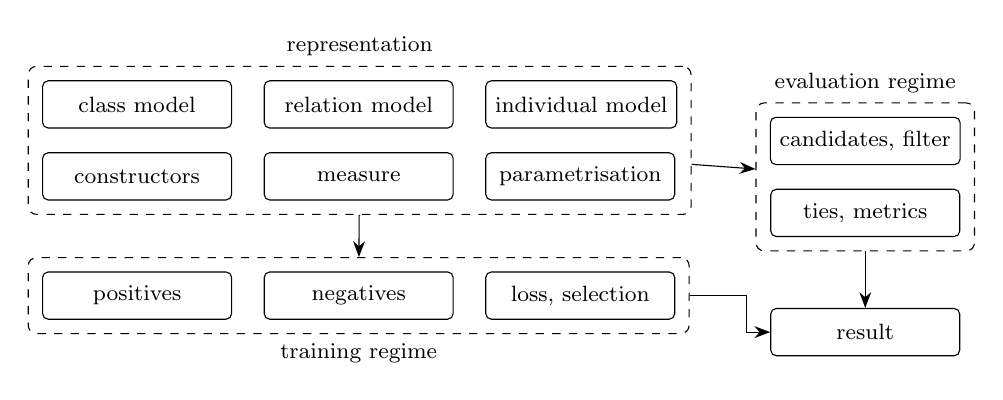
\begin{tikzpicture}[font=\footnotesize, node distance=3mm and 4mm,
  part/.style={draw, rounded corners=2pt, minimum height=6mm, minimum width=24mm, align=center},
  group/.style={draw, dashed, rounded corners=3pt, inner sep=5pt},
  arr/.style={-{Stealth[length=2mm]}}]
\node[part] (cls) {class model};
\node[part, right=of cls] (rel) {relation model};
\node[part, right=of rel] (ind) {individual model};
\node[part, below=of cls] (con) {constructors};
\node[part, right=of con] (mea) {measure};
\node[part, right=of mea] (par) {parametrisation};
\node[group, fit=(cls)(ind)(con)(par), label={[font=\footnotesize]above:representation}] (rep) {};
\node[part, below=9mm of con] (pos) {positives};
\node[part, right=of pos] (neg) {negatives};
\node[part, right=of neg] (loss) {loss, selection};
\node[group, fit=(pos)(loss), label={[font=\footnotesize]below:training regime}] (tr) {};
\node[part, right=12mm of par, yshift=4.5mm] (cand) {candidates, filter};
\node[part, below=of cand] (tie) {ties, metrics};
\node[group, fit=(cand)(tie), label={[font=\footnotesize]above:evaluation regime}] (ev) {};
\node[part, below=9mm of tie, minimum width=24mm] (res) {result};
\draw[arr] (rep) -- (tr);
\draw[arr] (rep) -- (ev);
\draw[arr] (tr.east) -| ([xshift=-3mm]res.west) -- (res.west);
\draw[arr] (ev) -- (res);
\end{tikzpicture}
\caption{The structure of a method in mOWL~3. The representation scores an axiom; a
training regime turns the scores of positive and negative axioms into a loss and selects
the epoch that is kept; an evaluation regime ranks the test axioms. Every box is an entry
of a registry and can be replaced without changing the others.}\label{fig:parts}
\end{figure}

\subsection{Training and evaluation regimes}

The procedure by which a method is trained and the procedure by which it is tested are
parts in the same sense. We read the experimental sections, the appendices and the
released code of the publications and named the procedures that recur. A training regime
fixes which axioms are positives (the asserted axioms, their deductive closure, or a
structure materialised by a reasoner), how negatives are produced (uniform corruption of
one or both sides, corruption filtered against the asserted axioms or against the
deductive closure, or axioms that are provably false), how scores are combined into a
loss, how batches are formed and which epoch is kept. An evaluation regime fixes the
candidates among which a test axiom is ranked, the axioms that are removed from the
ranking, the treatment of ties and the metrics. The catalogue contains 86 training
regimes and 40 evaluation regimes, each with the publication and the section or source
file from which it was taken. A regime is attached to a model independently of the
representation, so that, for example, the negatives of one publication can be used with
the regions of another.

Separating the regimes from the representations exposed differences between
publications that appear to report the same experiment. The benchmarks derived from the
Gene Ontology, GALEN and the Anatomy ontology are used by several publications, which
rank a test axiom among different candidate sets, filter different axioms and count ties
differently. mOWL~3 therefore records each such protocol as a separate evaluation regime
and names the benchmarks after the publication whose protocol they follow.

\subsection{Published behaviour and corrected behaviour}

Decomposing a published method into parts revealed places where the released code of a
method differs from its paper, and places where a paper prescribes a behaviour that is
an error by its own definitions, for example a loss for $C \sqcap D \sqsubseteq E$ that
mixes the axioms of a batch. mOWL~3 applies one rule to these cases. A method that is
requested by its published name behaves as its authors' implementation does, so that
published numbers remain reproducible. A part that is requested on its own has the
corrected behaviour as its default, and the published behaviour remains available as a
named option. The documentation lists each such deviation with the publication, the
location in the released code and the option that selects it.

\subsection{Expressivity, inference tasks and reasoners}

A method supports a fragment of OWL, and applying it to an ontology outside this
fragment silently discards axioms. mOWL~3 represents description logic expressivity as an
object in the standard notation, for example ``\ELpp{} with ABox''. Every method
states the expressivity that it supports, the expressivity that an ontology uses is
computed from its axioms, and a model reports at construction how many axioms of its
training ontology lie outside its fragment and which constructs they use. The inference
tasks are explicit in the same way: a method declares the tasks for which it gives a
score (subsumption, instance checking, role assertion, query answering and others), and
a benchmark declares the tasks that it requires. Reasoners are backends that are
selected by expressivity. mOWL~3 packages ELK for the \EL{} family and HermiT for OWL~2
DL through the OWL API~5~\cite{horridge2011}, and selects the cheapest reasoner that is
complete for the ontology at hand.

\section{The Method Catalogue}

The catalogue is the index of the methods. Each method has a card that records its
publication, the family to which it belongs, the description logic that it supports,
the inference tasks that it scores, its eight parts, whether the parts are independent,
and the model class that implements it. Table~\ref{tab:catalogue} summarises the 64
implemented methods by family. The geometric family is the largest and covers balls,
boxes, cones, ellipsoids, octagons, prisms and unions of boxes as class models. The
constructive family contains methods that compute an embedding from a canonical or least
model instead of training it, and that are used to test whether a class of geometric
models can represent a given ontology exactly.

\begin{table}[t]
\caption{The 64 methods of the catalogue by family, with examples.}\label{tab:catalogue}
\centering\footnotesize\setlength{\tabcolsep}{4pt}
\begin{tabular}{@{}lrp{8.0cm}@{}}
\toprule
Family & Methods & Examples \\
\midrule
Geometric & 32 & ELEmbeddings~\cite{kulmanov2019}, EmEL++~\cite{mondal2021},
  ELBE~\cite{peng2020}, BoxEL~\cite{xiong2022}, Box$^2$EL~\cite{jackermeier2024},
  TransBox~\cite{yang2025}, RegD~\cite{yang2025regd}, EIKE~\cite{wang2024eike},
  BoxLitE~\cite{lourenco2026},
  Concept2Box~\cite{huang2023}, Query2Box~\cite{ren2020q2b}, FaithEL~\cite{lacerda2024faithel} \\
Constructive & 9 & canonical and least models, exact cone models for \ALC{}~\cite{ozcep2023},
  exact box models by integer programming \\
Order & 7 & order embeddings~\cite{vendrov2016}, box lattice~\cite{vilnis2018},
  hyperbolic cones~\cite{ganea2018}, CatE~\cite{zhapa2023} \\
Graph & 7 & DL2Vec~\cite{chen2020}, OWL2Vec*~\cite{chen2020b}, projection with
  knowledge graph embeddings \\
Algebraic & 3 & E2R~\cite{garg2019}, BetaE~\cite{ren2020betae} \\
Fuzzy & 2 & FALCON~\cite{falcon2022}, DF-\ALC~\cite{wu2022} \\
Language model & 2 & HiT~\cite{he2024hit}, OnT~\cite{yang2025ont} \\
Syntactic & 2 & Onto2Vec~\cite{smaili2018}, OPA2Vec~\cite{smaili2019} \\
\bottomrule
\end{tabular}
\end{table}

The catalogue can be queried by any field of a card. A user who has an ontology can ask
which methods support its expressivity; a user who needs instance checking can ask which
methods score it; and the methods that share a part can be listed, for example all
methods whose classes are boxes together with their relation models. The same queries
select the methods that are offered for a benchmark: a benchmark whose test data name
classes that training did not see is offered only to methods whose embeddings are
computed from text or from a graph.

\section{The Benchmark Set}

\subsection{Benchmarks, published numbers and recipes}

A benchmark in mOWL~3 consists of a dataset with its split, an evaluation regime, the
form of the axioms that are ranked, and a statement of which axioms count as correct:
those that were held out, or those that the training ontology entails. The set contains
124 benchmarks in seven groups (Table~\ref{tab:benchmarks}). Most are the benchmarks of
publications, with the data of the publication and the evaluation regime that was read
from its paper and code.

\begin{table}[t]
\caption{The benchmarks of mOWL~3 by task group.}\label{tab:benchmarks}
\centering\footnotesize\setlength{\tabcolsep}{4pt}
\begin{tabular}{@{}lrp{6.6cm}@{}}
\toprule
Task group & Benchmarks & What is scored \\
\midrule
Axiom prediction & 30 & held-out class inclusions of an ontology \\
Exact model & 29 & whether the trained embedding is a model of the ontology \\
Link prediction & 28 & held-out role assertions or axioms $C \sqsubseteq \exists r.D$,
  for example protein--protein interactions \\
Deductive inference & 23 & entailed class inclusions, ranked above those that are not entailed \\
Query answering & 7 & answers of one-hop and multi-hop logical queries \\
Membership prediction & 5 & held-out class assertions \\
Faithfulness & 2 & agreement of the embedding with entailment and non-entailment \\
\bottomrule
\end{tabular}
\end{table}

For each benchmark, mOWL~3 records the numbers that publications report for it. A
published result consists of the method, the subset of the test data, the metric, the
value, the publication and the table and row in which the value is printed. The set
contains 1,007 such values from 25 publications. A recipe records how a publication
trained a method on a benchmark: the arguments of the model, the training regime with its
arguments, the number of epochs and the validation interval, together with a note on
every setting that the publication does not state or that differs between the paper and
its code. The set contains 871 recipes from 24 publications. With a recipe, one command
trains a method as its publication did and compares the result with the published
numbers:

\begin{lstlisting}[language=bash]
python -m mowl.benchmarks run box2el-go-prediction \
       --method box2el --recipe
\end{lstlisting}

\subsection{Joint benchmarks}

The numbers of two publications on the same data cannot be compared when their
evaluation regimes differ. mOWL~3 therefore adds joint benchmarks that apply one
evaluation regime, filtered ranking with mean ranks for ties, to the data that most
publications share: class inclusion prediction, existential restriction prediction and
subsumption inference on the Gene Ontology, GALEN and the Anatomy ontology, and
protein--protein interaction prediction for yeast and human. Every method that scores
the required task can be run on a joint benchmark. Table~\ref{tab:joint} shows a
selection. The values are from one seed with the default settings of each method and
without hyperparameter search; they show that methods from all families run under one
protocol and are a starting point for a tuned comparison.

\begin{table}[t]
\caption{Filtered MRR and AUC of a selection of methods on four joint benchmarks on the
Gene Ontology (GO) and on yeast protein--protein interactions (PPI): one seed, default
settings, no hyperparameter search. A dash marks a task that the method does not
score.}\label{tab:joint}
\centering\footnotesize\setlength{\tabcolsep}{4pt}
\resizebox{\textwidth}{!}{%
\begin{tabular}{@{}llcccc@{}}
\toprule
 & & GO subs. & GO subs. & GO exist. & Yeast \\
Method & Family & prediction & inference & prediction & PPI \\
\midrule
ELEmbeddings & geometric & 0.085 / 0.91 & 0.021 / 0.84 & 0.370 / 0.94 & 0.017 / 0.80 \\
ELBE & geometric & 0.057 / 0.88 & 0.028 / 0.91 & 0.112 / 0.86 & 0.018 / 0.77 \\
Box$^2$EL & geometric & 0.094 / 0.95 & 0.045 / 0.97 & 0.383 / 0.94 & 0.062 / 0.96 \\
TransBox & geometric & 0.057 / 0.88 & 0.004 / 0.74 & 0.148 / 0.93 & 0.001 / 0.42 \\
ELK-Em & geometric & 0.110 / 0.97 & 0.048 / 0.99 & 0.078 / 0.96 & 0.109 / 0.95 \\
BoxE & geometric & 0.184 / 0.97 & 0.119 / 0.98 & 0.132 / 0.96 & 0.224 / 0.97 \\
Order embeddings & order & 0.033 / 0.89 & 0.098 / 0.98 & -- & -- \\
Box lattice & order & 0.052 / 0.91 & 0.136 / 0.95 & -- & -- \\
CatE & order & 0.012 / 0.91 & 0.010 / 0.95 & -- & 0.079 / 0.86 \\
DL2Vec & graph & 0.094 / 0.95 & 0.050 / 0.99 & 0.102 / 0.97 & 0.194 / 0.97 \\
OWL2Vec* & graph & 0.087 / 0.96 & 0.053 / 0.98 & 0.092 / 0.97 & 0.188 / 0.97 \\
Onto2Vec & syntactic & 0.134 / 0.87 & 0.007 / 0.86 & 0.005 / 0.88 & 0.188 / 0.95 \\
FALCON & fuzzy & 0.002 / 0.75 & 0.003 / 0.91 & 0.001 / 0.47 & 0.001 / 0.59 \\
OnT & lang. model & 0.053 / 0.83 & 0.005 / 0.69 & 0.007 / 0.80 & 0.003 / 0.55 \\
\bottomrule
\end{tabular}}
\end{table}

\section{Reproduction Study}

\subsection{Design}

The decomposition into parts is useful only if a method assembled from parts computes
what the method computes. We tested this in two ways. First, for each method we kept an
independent direct implementation, written as one unit in the manner of the released
code, as a baseline. The baselines are part of mOWL~3 and are selected with a command
line option. Unit tests compare the loss of each axiom form between the parts and the
baseline on the same parameters. Second, we ran each method on its benchmarks with its
recipe, once from the parts and once with the baseline, and compared both results with
each other and with the published numbers. The study comprises 1,238 planned runs, of
which 1,170 are complete; 19 cannot be made, for reasons that we give in
Section~\ref{sec:limits}, and the remaining runs each need between one and several days.
A run uses one to three seeds, and the number of seeds of each value is recorded with it.

We report agreement on the metrics that take values between 0 and 1 (hits at $k$, mean
reciprocal rank, area under the curve, $F_1$ and accuracy), for which an absolute
difference has the same meaning across benchmarks. Mean ranks are in the full comparison
table of the documentation.

\subsection{Parts and direct implementations agree}

The first question is whether a method built from parts gives the result of its direct
implementation. Both implementations were run for 341 pairs of a method and a benchmark,
covering 29 methods, which gives 2,294 pairs of metric values
(Table~\ref{tab:agreement}). The median absolute difference is 0.001, and 76\% of the
values differ by at most 0.02. The unit tests establish that both implementations compute
the same loss from the same parameters, so that the larger differences arise during
training, where the two implementations can differ in the order in which they draw
initial parameters and negatives and in the epoch that they keep. The comparison table
of the documentation marks each value that differs by more than 2\%. The agreement of
the losses and of most trained results shows that the decomposition preserves the
methods.

\begin{table}[t]
\caption{Absolute differences between metric values in $[0,1]$: the method built from
parts against its direct implementation, and each implementation against the published
value.}\label{tab:agreement}
\centering\footnotesize\setlength{\tabcolsep}{4pt}
\resizebox{\textwidth}{!}{%
\begin{tabular}{@{}lrrrr@{}}
\toprule
Comparison & Values & Median & Within 0.02 & Within 0.05 \\
\midrule
Parts against direct implementation & 2,294 & 0.001 & 76\% & 83\% \\
Parts against published & 1,437 & 0.010 & 63\% & 79\% \\
Direct implementation against published & 1,427 & 0.022 & 48\% & 66\% \\
\bottomrule
\end{tabular}}
\end{table}

\subsection{Agreement with the published numbers}

The second question is whether mOWL~3 reproduces the published numbers. Published values
are available for 169 pairs of a method and a benchmark, covering 20 methods and 95
benchmarks, which gives 1,437 values with a counterpart from the parts. The median
absolute difference between the value from the parts and the published value is 0.010,
and 79\% of the values lie within 0.05 of the published value
(Table~\ref{tab:agreement}). The methods built from parts are closer to the published
numbers than the direct implementations: among the 1,419 values for which all three
numbers exist, the parts are closer in 745 cases, the direct implementation in 477, and
the two are equally close in 197. A likely reason is that the
training regimes of the parts were written from the publications and their code, while
the direct implementations keep the training loop of mOWL~2.1.0.

Table~\ref{tab:reproduction} summarises the outcome per method. We count a method as
reproduced when all its reported metrics agree with the publication within the variation
between seeds, and as partly reproduced when this holds for some of its benchmarks.

\begin{table}[t]
\caption{Reproduction of published results with the recipes of mOWL~3.}\label{tab:reproduction}
\centering\footnotesize\setlength{\tabcolsep}{4pt}
\begin{tabular}{@{}p{3.0cm}p{1.6cm}p{6.9cm}@{}}
\toprule
Method & Status & Remark \\
\midrule
Box$^2$EL~\cite{jackermeier2024} & reproduced & largest gap in Hits@100: 0.31 against 0.35 (GALEN prediction) \\
TransBox~\cite{yang2025} & reproduced & all normal forms \\
ELEm, EmEL++, ELBE & reproduced & as baselines of the Box$^2$EL publication \\
OnT~\cite{yang2025ont} & reproduced & all six benchmarks \\
BoxEL~\cite{xiong2022} & partly & one published value results from a ranking error in the reference code \\
HiT~\cite{he2024hit} & partly & four of six benchmarks \\
CatE~\cite{zhapa2023} & partly & two benchmarks reproduced; one depends on data that differ from the release \\
DELE~\cite{mashkova2024} & partly & most values within a few percent \\
RegD~\cite{yang2025regd} & partly & about half of 48 values within 0.04 $F_1$ \\
ELK-Em~\cite{singh2026} & partly & two of three ontologies \\
EmEL++~\cite{mondal2021} & partly & on its own benchmarks, close but below \\
Concept2Box~\cite{huang2023} & not reproduced & reported numbers require data that were not released \\
EIKE~\cite{wang2024eike} & not reproduced & 68 / 67 / 85 against 87 / 81 / 93 $F_1$ \\
BoxLitE~\cite{lourenco2026} & not reproduced & requires a commercial solver \\
\bottomrule
\end{tabular}
\end{table}

\subsection{Causes of differences}

A difference between a reproduced and a published number is informative when its cause
can be identified. Because the parts isolate each choice, we could trace several
differences to one cause, and we describe four of them.

The first cause is the rule that selects the training epoch. Up to version 2.1.0, a
model in mOWL kept the epoch with the lowest loss on the validation axioms. This loss is
computed on true axioms only. For several box models it is lowest before training has
separated true from false axioms, when all boxes still overlap and every inclusion holds.
In the first round of the joint benchmarks, 84 of 758 runs kept such an untrained state
and ranked at chance level, among them every run of BoxSEL and most runs of Concept2Box.
The selection rule is a part of the training regime, and mOWL~3 replaces it by a rule
that keeps the epoch at which the validation axioms score better than corrupted copies of
themselves most often. With this rule the area under the curve of BoxSEL on the affected
benchmarks rises from 0.50 to between 0.61 and 0.94. The selection rule is rarely stated
in publications, and this result shows that it can decide the outcome of a comparison.

The second cause is an undocumented training schedule. The publication of EIKE describes
classes as ellipsoids with trained axes. With its recipe mOWL~3 reaches $F_1$ values of 68,
67 and 85 on instance, subclass and relational triples of YAGO39K, against 87, 81 and 93
in the publication, while the authors' code reproduces the publication. The authors' code
keeps the axes fixed for the first 1,000 epochs, during which the classes are spheres.
When we fix the axes in mOWL~3 and use the initialisation of the authors' code, mOWL~3
gives 82 and 92 for instance and relational triples, in agreement with the authors' code
under the training loop of mOWL~3 (81 and 91). The subclass score remains lower (54
against 74) and its cause is open.

The third cause lies in the benchmark. On subsumption inference, Concept2Box and EIKE
reach an area under the curve of 0.93 and 0.81 on the Gene Ontology and of 0.52 and 0.54
on GALEN. Of the 16,325 inferred
test axioms of GALEN, 64 follow from the stated class hierarchy alone, compared with 60\%
of the test axioms of the Gene Ontology. The remaining test axioms of GALEN follow only
with definitions of the forms $C \sqcap D \sqsubseteq E$ and
$\exists r.C \sqsubseteq D$, and these two methods train on class inclusions and
existential restrictions only. The catalogue states this restriction for both methods,
and the benchmark states the forms that it requires.

The fourth cause is in the published numbers themselves. The instance-view results
reported for Concept2Box include a row for a baseline whose values are those of an
earlier publication on a larger dataset that was not released; on the released data this
baseline reaches a mean reciprocal rank between 0.09 and 0.16 against the reported 0.32.
For RegD with boxes, the code released by the authors, run with its own hyperparameter
sweep, reproduces the published numbers for the ball-based variants and gives 0.39
against the published 0.63 on inference over the Anatomy ontology; mOWL~3 is at or above
the released code. In both cases the recipe records the finding, so that a user who
compares against these numbers sees it.

\section{Use, Documentation and Availability}

\subsection{Use}

The entry point for a new user is one function that builds, trains and evaluates a
method (Listing~\ref{lst:pipeline}). It takes the name of a method and the name of a
benchmark and returns the trained model with its metrics. Given an ontology file in place
of a benchmark, it trains on the user's ontology, optionally with the evaluation regime
of a named benchmark applied to the user's own validation and test ontologies. A result
can be written to a directory and loaded again with its model. The function starts the
Java virtual machine that the OWL API requires, so that no setup precedes the call.

\begin{lstlisting}[language=Python,caption={Training and evaluating a method on a
benchmark and on a user's ontology.},label=lst:pipeline,float=t]
from mowl.pipeline import pipeline, load_pipeline

result = pipeline("box2el", benchmark="box2el-go-prediction",
                  recipe=True)
print(result.metric("mrr"))
result.save_to_directory("box2el_go")
model = load_pipeline("box2el_go").model

mine = pipeline("elem", dataset="my_ontology.owl", epochs=200)
\end{lstlisting}

A trained model answers the same questions whatever its method: the score of an axiom,
the region of a class, and the classes that lie inside a compound class expression. A new
class model, relation model, measure, training regime or evaluation regime is added by
registering it, after which it can be combined with the existing parts; a new method is
a card and a tuple of parts; and a new benchmark is a dataset, an evaluation regime and,
if available, its published numbers and recipes.

\subsection{Quality and documentation}

mOWL~3 has about 5,800 unit tests that run on each change for four Python versions.
Among them are tests that compare each method built from parts with its direct
implementation, tests of the public interface of the previous release, and behaviour
tests that record what mOWL computes from four fixture ontologies (signature, normal
forms, projections, reasoner answers) and that guard changes of the Java libraries; they
were used to move mOWL from the OWL API~4 to the OWL API~5. The documentation contains a
tutorial for the first steps, a page for each method that states what was read from the
paper and what from the code, the catalogue, the benchmark set with the published
numbers, and the comparison tables of the reproduction study. Its 214 code examples are
executed in continuous integration.

\subsection{Availability and sustainability}

mOWL is developed in a public GitHub repository\footnote{\url{https://github.com/bio-ontology-research-group/mowl}}
under the BSD 3-Clause license and is distributed through the Python Package Index as \texttt{mowl-borg}.
 The project follows semantic versioning.
Because mOWL~3 changes default behaviour, it is a major release, and its changelog states
for each changed default how the behaviour of version 2.1.0 is obtained. Releases are
made on a quarterly schedule, with patch releases for defects in between, and
dependencies are updated automatically each week. mOWL has been maintained by the
Bio-Ontology Research Group since its first release. 

\section{Limitations and Conclusion}\label{sec:limits}

The reproduction study has limits that a user of its numbers should know. Sixty-eight of
the 1,238 planned runs are absent from the tables. Nineteen of them cannot be made:
the canonical model on which FaithEL is defined would have between $3 \times 10^8$ and
$6 \times 10^9$ elements for the ontologies of the joint benchmarks, the Statistical
\EL{} ontologies of BoxSEL were not released, and one query set is not redistributable.
The others are query answering on large knowledge graphs and Monte Carlo ranking on the
large ontologies, each of which needs between one and several days, and they can be added
without changes to the code. Most values come from one seed, so that small differences
between methods in Table~\ref{tab:joint} are within the variation that further seeds
would show. For one fifth of the published values, mOWL~3 differs by more than 0.05, and
for some of them, including the subclass score of EIKE, we have found no cause. Each of
these cases is listed on the reproduction page of the documentation with the experiment
that would settle it.

mOWL~3 changes what can be asked of ontology embedding methods. Because a method is a
combination of parts with a training regime and an evaluation regime, a claimed
improvement can be tested by exchanging one part under a fixed protocol, and the
combinations that no publication has tested can be run with one line of code. The
catalogue states for each method which description logic and which inference tasks it
supports, and the benchmark set records what was published, under which protocol, and
with which configuration. The reproduction study shows that the parts preserve the
methods and that most published numbers are reproduced, and it traces several of the
remaining differences to choices that publications leave unstated, such as the rule that
selects the training epoch. We plan to complete the long runs, to add seeds to the joint
benchmarks, and to use the joint benchmarks for a comparison of all methods under equal
tuning budgets.

\begin{credits}


\subsubsection{\discintname} The authors have no competing interests to declare that are
relevant to the content of this article.
\end{credits}

\bibliographystyle{splncs04}
\bibliography{references}

\end{document}
